\chapter{Array SSA Form \Author{V. Sarkar \andAuthor K. Knobe \andAuthor S. Fink}}
\label{chapter:array_ssa}
\inputpath{part2}{array_ssa}
\inputprogress
\ssainput{part2/array_ssa}{preamble}
%% \newcommand\REM[1]{REM:#1}
%% \def\REM{REM:}
%% \newenvironment{programa}{\begin{minipage}{0.6\textwidth}
%% }{%
%% \end{minipage}}
%% \def\Ta{\hspace{1em}}
%% \def\Tb{\hspace{2em}}
%% \def\Tc{\hspace{3em}}
%% \def\Td{\hspace{4em}}
%% \def\Te{\hspace{5em}}
%% \def\False{\textsf{False}}
%% \def\True{\textsf{True}}
%% \def\Set{\textsf{Set}}
%% \def\U{U}
%% \def\URS{URS}
%% \def\DRS{DRS}
%% \def\DDS{DDS}
%% \def\DDRS{DDRS}
%% \def\DEAD{DEAD}
%% \def\KILL{KILL}
%% \def\LIVE{LIVE}
%% \def\imp{imp}
%% \def\DS{DS}
%% \def\ds{ds}
%% \def\DD{DD}
%% \def\dd{dd}
%% \def\viz{viz}
%% \def\Update{Update}
%% \def\Valnum{Valnum}
%% \def\No{No}
%% \def\Maybe{Maybe}
%% \def\Must{Must}
%% \def\Yes{Yes}
%% \def\X{X}
%% \def\T{T}
%% \def\F{F}
%% \def\L{L}
%% \def\H{H}
%% \def\V{V}
%% \def\HA{HA}
%% \def\Hb{Hb}
%% \def\Hc{Hc}
%% \def\Hd{Hd}
%% \def\Hf{Hf}
%% \def\Hi{Hi}
%% \def\Hl{Hl}
%% \def\HO{HO}
%% \def\At{At}
%% \def\jp{jp}
%% \def\joc{joc}

\label{sec:intro}
In this chapter,
we introduce an Array SSA form 
that captures element-level data-flow information for array variables, and
coincides with standard SSA form when applied to scalar variables.  
Any program with arbitrary control-flow structures and arbitrary array
subscript expressions can be automatically converted to this 
Array SSA form, thereby making it applicable to structures, heap
objects and any other data structure
that can be modeled as a logical array.
A key extension over standard SSA form is the introduction of a
{\em definition-$\Phi$} function that is capable of
merging values from distinct array definitions on an element-by-element
basis. 
There are several potential applications of Array SSA form in compiler
analysis
and optimization of sequential and parallel programs.
In this chapter, we focus on sequential programs and use
{\em constant propagation}
as an exemplar of a program analysis that can be extended to array variables
using Array SSA form, and {\em redundant load elimination} as an
exemplar  of a program optimization that can be extended to heap objects using Array SSA form.
% As with many algorithms based on scalar SSA form, the algorithms presented in this chapter are linear in the size of the Array SSA form representation.
% Though Array SSA form can be made manifest at run-time (\eg\ when enabling parallelization via storage duplication~\cite{KnSa98}), all the algorithms described in this chapter  use Array SSA form as a basis
% for program analysis, 
% which means that the Array SSA form
% structures can be removed after the  program properties
% of interest
% have been discovered.

The rest of the chapter is organized as follows.
Section~\ref{sec:arrayssa} introduces {\em full Array SSA form} for run-time
evaluation and {\em partial Array SSA form}
for static analysis.  
Section~\ref{sec:cp} extends the scalar SSA
constant propagation algorithm to enable
constant propagation through array elements.
This includes an extension to the constant
propagation lattice to efficiently
record information about array
elements and an extension to the
work-list algorithm to support  {\em definition-$\Phi$} functions (section~\ref{sec:arraylattice}), and
a further extension to support non-constant (symbolic) array
subscripts (section~\ref{sec:non-const}). 
Section~\ref{sec:heap} shows how Array SSA form can be extended to
support elimination of redundant loads of 
object fields and array elements in strongly typed languages,
and section~\ref{sec:conclusions} contains suggestions for further reading.

\section{Array SSA form}
\label{sec:arrayssa}
% TODO:
% 1) Replace earlier Array SSA example by the same one used for
% constant propagation

% The goal of Array SSA form is to provide the same benefits for arrays
% and related data structures
% that traditional SSA form provides for scalars.
% Section~\ref{sec:full} summarizes  {\it full Array SSA form}, which provides exact use-def information 
% at run-time for each dynamic access of an array element.
% Section~\ref{sec:partial} introduces {\it partial Array SSA form} as a
% static approximation of full Array SSA form.
% Throughout this chapter,
% we assume that all array operations in the input program are
% expressed as reads and writes of individual array elements.  The
% extension to more complex data structures such as arrays of
% structures and nested arrays 
% has been
% omitted to simplify the presentation of this chapter.

%\subsection{Full Array SSA Form}\label{sec:full}

% The full Array SSA form uses $\Phi$ operators instead of $\phi$
% functions used by traditional SSA form. The semantics of the $\Phi$
% operator can be defined as a pure function.  
% This is one respect in which Array SSA form
% has
% advantages over traditional SSA form even for scalar variables.
% {\it @ variables} (pronounced ``at variables'')
% are used to obtain a pure function semantics for the
% $\Phi$
% operator. Each
% $\phi$ function in traditional SSA form such as $\phi(S_1,S_2)$ is
% rewritten as $\Phi(S_1,@S_1,S_2,@S_2)$.  

To introduce full Array SSA form with runtime evaluation of $\Phi$
functions,
we use the concept of an  {\it iteration vector} to differentiate among multiple dynamic
instances of a static definition, $S_k$, that occur in the same
dynamic instance of $S_k$'s enclosing procedure, $f()$.
% The {\it iteration vector} of a 
% static 
% definition $S_k$ identifies a single iteration in the iteration space of the
% set of loops
% that enclose the definition. 
Let $n$ be the number of loops that enclose $S_k$ in procedure $f()$.
These loops could be for-loops, while-loops, or even loops constructed
out of goto statements.
For convenience, we treat the outermost
region of acyclic control flow in a procedure as a dummy outermost loop
with a single iteration, thereby ensuring that $n \geq 1$.

A single point in the
iteration space is specified by the iteration vector
$\vec{i} = (i_1, \ldots, i_n)$, which is
an 
$n$-tuple of iteration numbers,
<one for each enclosing loop. 
For convenience, this definition of iteration vectors assumes that  
all loops are single-entry, or equivalently, that the control-flow graph is {\it reducible}.
(This assumption is not necessary
for partial Array SSA form.)
For single-entry loops, we know that each def executes at most
once in a given iteration of its surrounding loops, hence the iteration vector
serves the purpose of a ``timestamp''.
The key extensions in Array SSA form relative to standard SSA form are as
follows.



\begin{enumerate}
\item {\bf Renamed array variables:}
All array variables are renamed so as to 
satisfy the static single assignment property.  Analogous to standard SSA
form, control $\Phi$ operators are introduced to generate new names
for merging two or more prior definitions at control-flow join points, and to ensure that each use
refers to precisely one definition.

\item {\bf Array-valued @ variables:}
For each static definition
$A_j$, we introduce an {\em @ variable} (pronounced ``at variable'')
$@A_j$ that identifies
the most recent {\em iteration vector} {\it
at} which definition $A_j$ was executed.
We assume that all @ variables are initialized to the empty
vector, $ (\;)$, at the start of program execution.  
% For each
% real (non-$\Phi$) definition of a renamed scalar, $S_k$, we assume that a statement of the
% form $@S_k := \vec{i}$ is inserted immediately after definition
% $S_k$, where $\vec{i}$
% is the current iteration vector for all loops that surround
% $S_k$. 
% All @ variables are initialized
% to the empty vector because the empty vector is the identity element
% for a lexicographic $\max$ operation \ie\ $\max((\;),\vec{i}) =
% \vec{i}$, for any @ variable value $\vec{i}$.
% Each  array variable, $A_j$, in Array SSA form has an associated 
% @ variable, $@A_j$, such that $@A_j$ has
% the same shape (rank and dimension sizes) as array variable $A_j$.
Each update of a single array element, $A_j[k] := \ldots$, 
is followed by the statement, $@A_j[k] := \vec{i}$
where $\vec{i}$ is the iteration vector for the loops surrounding
the definition of $A_j$.
% Thus, an array-valued @ variable, $@A_j$,  
% can record a separate iteration vector for
% each element that is assigned by definition $A_j$.


\item {\bf Definition $\Phi$'s:}
\label{def:phi}
A  {\it definition}-$\Phi$ operator is 
introduced in Array SSA form to deal with preserving (``non-killing'') definitions
of arrays.  Consider $A_0$ and $A_1$, two renamed 
arrays that originated from the same array variable in the source program
such that $A_1[k] := \ldots$
is an update of a single array element
and $A_0$ is the prevailing definition at the program point just
prior to the definition of $A_1$.
A definition $\Phi$, $A_2 := d\Phi(A_1, @A_1, A_0, @A_0)$,
is inserted immediately after the definitions for $A_1$ and $@A_1$.
% (We use the notation $d\Phi$ when we want to 
% distinguish a definition $\Phi$ operator from a control $\Phi$ operator.)
Since definition $A_1$ only updates one element of $A_0$, $A_2$ represents
an element-level merge of arrays $A_1$ and $A_0$.
Definition $\Phi$'s did not need to be
inserted in standard SSA form because a scalar definition completely kills the old value of
the variable.  


\item {\bf Array-valued  $\Phi$ operators:}
\label{array:phi}
Another consequence of renaming arrays is that
a $\Phi$ operator
for array variables must also return an
array value.  Consider a (control or definition) $\Phi$ operator of
the form, $A_2 := \Phi(A_1, @A_1, A_0, @A_0)$. Its semantics can be specified precisely
by the following conditional expression
for each element, $A_2[j]$, in the result array $A_2$:
\begin{eqnarray}
A_2[j] & = &
  \begin{array}{llll}
\mbox{\bf if} & @A_1[j] \succeq @A_0[j] & \textbf{then} & A_1[j] \\
\mbox{\bf else} & A_0[j] \\
\mbox{\bf end if} \label{eqn:cond-expr}
  \end{array}
\end{eqnarray}
The key extension over the scalar case is that the conditional expression
specifies an element-level merge of arrays $A_1$ and $A_0$.
\end{enumerate}





Figures~\ref{fig:ssa-acyclic-array} and \ref{fig:full-form}
show an example program with an
array variable, and the conversion of the program to full Array SSA form as
defined above.

\begin{figure}%[p]
\begin{center}
\parbox{3.0in}{
\begin{programa}
%\mbox{n1:}
\Tb $A[*] := \mbox{\rm initial value of $A$}$\\
\Tb$i := 1$ \\
\Tb $C := i\ <\ 2 $\\
\Tb if $C$ then \\
%\mbox{n2:}
\Tc $k := 2\ *\ i$ \\
\Tc $A[k] := i$\\
\Tc print $A[k]$\\
\Tb endif \\
%\mbox{n3:}
\Tb print $A[2]$
\end{programa}
}\\
\end{center}
\caption{Example program with array variables}
\label{fig:ssa-acyclic-array}
\end{figure}


\begin{figure}%[p]
\begin{center}
\parbox{3.0in}{
\begin{programa}
%\mbox{n1:}
%\Tb $@i := (\;)$ ; $@C := (\;)$ ; $@k := (\;)$ ; \\
\Tb $@A_0[*] := (\;)$ ; $@A_1[*] := (\;)$\\
\\
\Tb $A_0[*] := \mbox{\rm initial value of $A$}$\\
\Tb $@A_0[*] := (1)$\\
\Tb $i := 1$ \\
%\Tb $@i := (1)$ \\
\Tb $C := i\ <\ n $ \\
%\Tb $@C := (1)$ \\
\Tb if $C$ then \\
%\mbox{n2:}
\Tc $k :=  2\ *\ i$ \\
%\Tc $@k := (1)$ \\
\Tc $A_1[k] := i$\\
\Tc $@A_1[k] := (1)$\\
\Tc $A_2 := d\Phi(A_1, @A_1, A_0, @A_0)$\\
\Tc $@A_2 := \max(@A_1, @A_0)$\\
\Tc print $A_2[k]$\\
\Tb endif \\
%\mbox{n4:} 
\Tb $A_3 := \Phi(A_2, @A_2, A_0, @A_0)$\\
\Tb $@A_3 := \max(@A_2, @A_0)$\\fig:
\Tb print $A_3[2]$ 
\end{programa}
}
\end{center}
\caption{Conversion of program in figure \protect{\ref{fig:ssa-acyclic-array}} to Full Array SSA Form}
\label{fig:full-form}
\end{figure}

We now introduce a {\it partial Array SSA form} for static analysis,
that serves as an approximation of full Array SSA form.
Consider a (control or definition) $\Phi$ statement, $A_2 := \Phi(A_1, @A_1, A_0, @A_0)$.
A static analysis will need to 
approximate
the computation of this $\Phi$ operator by 
some data-flow transfer function, $\L_{\Phi}$.
The inputs and output of $\L_{\Phi}$ will be
{\it lattice elements} for scalar/array variables that
are compile-time approximations of their run-time values.
We use the notation $\L(V)$ to denote the lattice element for 
a scalar or array
variable $V$.
Therefore, the 
statement, $A_2 := \Phi(A_1, @A_1, A_0, @A_0)$, will in general
be modeled by the data-flow equation,
$\L(A_2) = \L_{\Phi}(\L(A_1), \L(@A_1), \L(A_0), \L(@A_0))$.

While the  {\em runtime} semantics of 
$\Phi$ functions for array variables critically depends on @ variables (Equation~\ref{eqn:cond-expr}),
many {\em compile-time analyses} do not need the full generality of @ variables.  
For analyses that do not distinguish among iteration instances,
it is sufficient to model
$A_2 := \Phi(A_1, @A_1, A_0, @A_0)$ by
a data-flow equation, $\L(A_2) = \L_{\phi}(\L(A_1), \L(A_0))$,
that does not use lattice variables $\L(@A_1)$ and $\L(@A_0)$.
For such cases, a {\it partial}
Array SSA form can be obtained by dropping 
dropping @ variables, and using the
$\phi$ operator, $A_2 := \phi(A_1, A_0)$ instead of
$A_2 := \Phi(A_1, @A_1, A_0, @A_0)$.  
A consequence of dropping @ variables is that partial Array
SSA form does not need to deal with iteration
vectors, and therefore does not require the control-flow graph to be {\it reducible} as in full Array SSA form.
For scalar variables, the resulting $\phi$ operator obtained by
dropping @ variables exactly coincides with standard SSA form.
% The use of $\phi$ operators without @ variables brings
% partial Array SSA form closer to traditional SSA form.
% The key difference is that partial Array SSA form still contains 
% renamed arrays and definition $\phi$ operators for updates to array elements.



% Our first observation is that there is no extra information
% provided at compile-time by the @ variables
% for any static analysis that does not distinguish between reachable code
% and unreachable code.  In such cases,
% it is sufficient to model
% $A_2 := \Phi(A_1, @A_1, A_0, @A_0)$ by
% a data-flow equation of the form $\L(A_2) = \L_{\phi}(\L(A_1), \L(A_0))$
% that does not use lattice variables $\L(@A_1)$ and $\L(@A_0)$.
% For array variables, the only useful information
% provided by an @ variable, $@A_1$ (say), at compile-time is an indication
% of which elements were updated by the assignment to array $A_1$.  
% %The actual ``timestamp'' (iteration vector) for the assignment is not
% %relevant if all paths are considered to be reachable.
% However, as we will see in section~\ref{sec:arraylattice}, this information
% is also included in the lattice value $\L(A_1)$ for array $A_1$. 

% Our second observation is that
% a static analysis that needs to distinguish between unreachable
% code and reachable code can do so efficiently
% by introducing {\it executable flags} for nodes and edges in the
% CFG (Control-flow Graph) as i.
% If executable flags are computed in the data-flow analysis, then
% the @ variables again do not provide any useful extra information.
% In fact, if we consider a control $\Phi$ statement
% $A_2 := \Phi(A_1, @A_1, A_0, @A_0)$, with array values $A_1$ and $A_0$
% carried by incoming CFG edges $e1$ and $e0$ respectively, then
% the corresponding data-flow equation (in the presence of unreachable code
% elimination) will be 
% $\L(A_2) = \L_{\Phi}(\L(A_1), X_{e1}, \L(A_0), X_{e0})$ where 
% $X_{e1}$ and $X_{e0}$ are the executable flags for edges $e1$ and $e0$.
% (Full details can be found i.)

% Since @ variables need not be modeled for the
% compile-time analyses discussed in this chapter,
% we drop them and use the
% $\phi$ operator, $A_2 := \phi(A_1, A_0)$ instead of
% $A_2 := \Phi(A_1, @A_1, A_0, @A_0)$ in {\it partial}
% Array SSA form.  
% A consequence of dropping @ variables is that partial Array
% SSA form does not need to deal with iteration
% vectors, and therefore does not require the control-flow
% graph to be {\it reducible} as in full Array SSA form.
% The use of $\phi$ operators without @ variables brings
% partial Array SSA form closer to traditional SSA form.
% The key difference is that partial Array SSA form still contains 
% renamed arrays and definition $\phi$ operators for updates to array elements.


\section{Sparse constant propagation of array elements}\label{sec:cp}
\subsection{Array lattice for sparse constant propagation }
\label{sec:arraylattice}
% Constant propagation for scalar variables has historically been performed
% by efficient data-flow analysis
% or
% abstract interpretation techniques in which values of variables are
% modeled as {\it lattice elements}~\cite{Kild73,WZ91}.
% Given a scalar variable $v$,
% the usual approach is to allow
% the value of its lattice element
% $\L(v)$ to be $\top$, $Constant$ or
% $\bot$.  When $\L(v)$ is $Constant$, the lattice
% element also contains the value of
% the constant\footnote{
% An extension that is sometimes employed is to also include
% lattice elements that can represent a
% small set of constants or a range of constants\cite{Harr77}.
% This functionality is not addressed in our chapter, but would be
% a straightforward extension to our framework.}.

% Formally, a lattice used for scalar constant
% propagation consists of:
% \begin{enumerate}
% \item A set of lattice elements:
% a lattice element for a program variable $v$ is written
% as $\L(v)$, and denotes $\Set(\L(v))$~=~a set of possible values for
% variable $v$.

% \item $\top$ (``top'') and $\bot$ (``bottom''), two distinguished
% elements of $\L$.
% The sets denoted by these lattice elements are
% $\Set(\top) = \{\;\}$ (the empty set), and $\Set(\bot) = \U^v$,
% where $\U^v$ is the universal set of values for variable
% $v$.
% \item  If $\L(v)$ is a $Constant$ lattice element
% $\Set(\L(v)) = \{Constant\}$, the singleton set containing a constant.
% \item A {\it join}
% operator, $\sqcap$, such that for any lattice element $e$,
% $e \sqcap \top = e$ and $e \sqcap \bot = \bot$. 

% The $\sqcap$ operator on lattice elements corresponds to the set {\it union}
% operation on the sets denoted by lattice elements
% \ie\ if $e$ and $f$ are two lattice elements, then 
% $\Set(e \sqcap f) = \Set(e) \cup \Set(f)$.

% It follows that the $\sqcap$
% operator is idempotent, commutative, and associative, and 
% that the lattice is {\it complete} \ie\ $\sqcap$ is closed
% on $\L$.
% \item A $\sqsupseteq$ operator such that $e \sqsupseteq f$ if and only if
% $e \sqcap f = f$, and a $\sqsupset$ operator such that $e \sqsupset f$
% if and only if $e \sqsupseteq f$ and $e \not= f$.

% The $\sqsupseteq$ and $\sqsupset$ operators on lattice elements
% correspond to the {\it inclusive subset} and {\it proper subset}
% operations on the sets denoted by lattice elements \ie\
% $e \sqsupseteq f$ if and only if $\Set(e) \subseteq \Set(f)$, and
% $e \sqsupset f$ if and only if $\Set(e) \subset \Set(f)$.

% The $\sqsupset$ operator defines a partial order on lattice elements.
% If $e \sqsupset f$, we say that $e$ is ``above'' $f$ and that $f$ is ``below''
% $e$ in the lattice.  Hence, $\top$ is above all other lattice elements
% and $\bot$ is below all other lattice elements.
% \end{enumerate}
% The {\it height} $H$ of lattice $\L$ is the length of the largest 
% sequence of lattice elements $e_1, e_2, \ldots, e_H$ such that
% $e_i \sqsupset e_{i+1}$ for all $1 \leq i < H$. The height of the
% lattice for scalar constant propagation is 3.


% We now describe how lattice elements for array variables are represented in 
% our framework for constant propagation.

In this section, we describe the lattice representation used to model
array values for constant propagation.
Let $\U^A_{ind}$ and $\U^A_{elem}$ be the universal set of {\it index values}
and the universal set of array {\it element values} respectively
for an array variable $A$.
For an array variable,
the set denoted by
lattice element $\L(A)$ is a subset of index-element pairs in $\U^A_{ind} \times \U^A_{elem}$.
There are three kinds of lattice elements for array variables that are of
interest in our framework:
\begin{enumerate}
\item $\L(A) = \top \;\;\imp\;\; \Set(\L(A)) = \{\;\}$\\
This ``top'' case indicates that the set of possible index-element
pairs
that have been identified thus far for $A$ is the empty set, $\{\;\}$.


\item $\L(A) = \langle(i_1,e_1), (i_2,e_2), \ldots\rangle$\\
$\imp\;\; \Set(\L(A)) = \{ (i_1,e_1), (i_2,e_2), \ldots \} \;\cup\;
(\U^A_{ind}-\{i_1,i_2,\ldots\})\times \U^A_{elem}$\\
The lattice element for this ``constant'' case is represented by a finite
list
of constant index-element pairs, $\langle(i_1,e_1), (i_2,e_2), \ldots\rangle$.
% where $i_1, i_2, \ldots$ are constant index values, and 
% $e_1, e_2, \ldots$ are constant element values.
The constant indices, $i_1, i_2, \ldots$, must represent distinct (non-equal)
index values.  
% The lattice ordering ($\sqsupset$) for these  elements is determined by the subset
% relationship among the sets that they denote.
The meaning of this lattice element is
that the current stage of analysis
has identified some finite number of constant index-element pairs
for array variable $A$, such
that $A[i_1] = e_1$, $A[i_2] = e_2$, etc.
All other elements of $A$ are assumed to be non-constant.
(Extensions to handle non-constant indices are
described in section~\ref{sec:non-const}.)

\item $\L(A) = \bot \;\;\imp\;\; \Set(\L(A)) =  \U^A_{ind} \times \U^A_{elem}$\\
This ``bottom''
case indicates that, according to
the approximation in the current stage of analysis, array $A$ may take on any
value from the universal set of index-element pairs.
Note that $\L(A)=\bot$ is equivalent to an empty list,
$\L(A)=\langle \; \rangle$, in case (2) above; they both 
denote the universal set of index-element pairs.
\end{enumerate}

% \begin{figure}%[tbp]
% \centerline{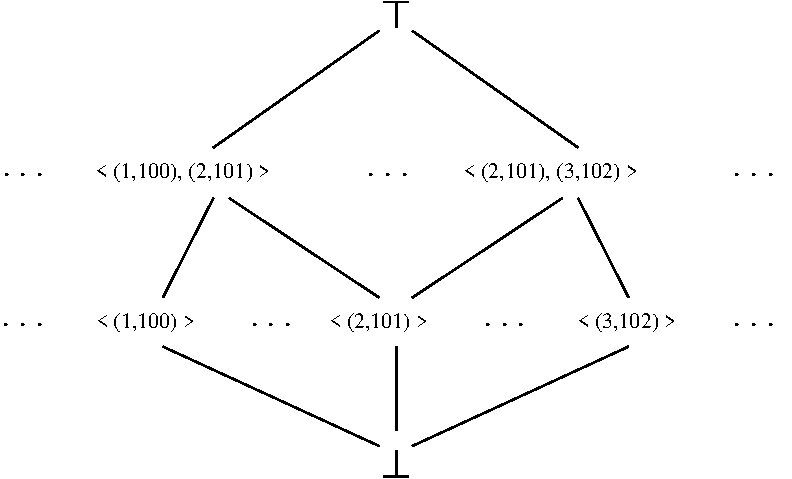
\includegraphics{array2.pdf}}
% \caption{Lattice elements of array values with maximum list size \protect{$Z=2$}}
% \label{fig:array2}
% \end{figure}

% Regardless of the size of an array, $A$, the number
% of index-element pairs in  $\L(A)$ is bounded by the number of
% static assignments to $A$ in the source. 
% We also 
% Since teh height of teh lattice is bounded by the maximu size of the
% list of constant index-element pairs,

% For the sake of efficiency, we will further restrict the constant array lattice
% elements, $\L(A) = \langle(i_1,e_1), (i_2,e_2), \ldots\rangle$,
% to lists that are bounded in size by some constant, $Z\geq 1$.
% The lattice structure for the $Z=2$ case is shown in figure~\ref{fig:array2}.  This lattice has four levels.  The second level (just below $\top$)
% contains all possible 
% lists that contain exactly two constant index-element pairs.  The third level (just above $\bot$) contains all possible 
% lists that contain a single constant index-element pair.  
% As mentioned earlier,
% the lattice ordering is determined by the subset relationship among the sets denoted by the lattice elements.  For example, consider two lattice elements $\L_1 = \langle(1,100), (2,101)\rangle$ and $\L_2 = \langle(2,101)\rangle$.  The sets denoted by these lattice elements are:
% \begin{eqnarray*}
% \Set(\L_1) & = & \{(1,100), (2, 101)\} \;\cup\;\;
% (\U_{ind} - \{1,2\}) \times \U_{elem} \\
% \Set(\L_2) & = & \{(2, 101)\} \;\cup\;\;
% (\U_{ind} - \{2\}) \times \U_{elem}
% \end{eqnarray*}
% Therefore, $\Set(\L_1)$ is a proper subset of $\Set(\L_2)$ and we have $\L_1 \sqsupset \L_2$ \ie\ $\L_1$ is above $\L_2$ in the lattice in figure~\ref{fig:array2}.


\begin{figure}%[htbp]
\begin{center}
\begin{tabular}{|l||c|c|c|}
\hline
$\L(A_1[k])$ & $\L(k) = \top$ & $\L(k) = Constant$ & $\L(k) = \bot$ \\
\hline \hline
$\L(A_1) = \top$ & $\top$ & $\top$ & $\bot$ \\
\hline
$\L(A_1) = \langle (i_1,e_1), \ldots \rangle$ & $\top$ & $e_j$, 
if $\exists$
$(i_j,e_j) \in \L(A_1)$ with &\\
& & $\DS(i_j, \L(k)) = \mbox{\it true}$ & $\bot$\\
& & $\bot$, otherwise & \\
\hline
$\L(A_1) = \bot$ & $\bot$ & $\bot$ & $\bot$ \\
\hline
\end{tabular}
\end{center}
\caption{Lattice computation for \protect{$\L(A_1[k]) = \L_{[\:]}(\L(A_1), \L(k))$},
where $A_1[k]$ is an 
array element read operator}
\label{fig:aref}
\end{figure}

\begin{figure}%[htbp]
\begin{center}
\begin{tabular}{|l||c|c|c|}
\hline
$\L(A_1)$ & $\L(i) = \top$ & $\L(i) = Constant$ & $\L(i) = \bot$ \\
\hline \hline
$\L(k) = \top$ & $\top$ & $\top$ & $\bot$ \\
\hline
$\L(k) = Constant$ & $\top$ & $\langle(\L(k),\L(i))\rangle$ & $\bot$ \\
\hline
$\L(k) = \bot$ & $\bot$ & $\bot$ & $\bot$ \\
\hline
\end{tabular}
\end{center}
\caption{Lattice computation for \protect{$\L(A_1) = \L_{d[\:]}(\L(k), \L(i))$},
where $A_1[k] := i$ is an 
array element write operator}
\label{fig:adef}
\end{figure}

We now describe how array lattice elements are computed for various
operations that appear in Array SSA form.  We start with the simplest operation
\viz\ a read access to an array element.
Figure~\ref{fig:aref} shows how $\L(A_1[k])$, the lattice element for array
reference $A_1[k]$, is computed as a function of $\L(A_1)$ and $\L(k)$, 
the lattice elements for $A_1$ and $k$.
We denote this function
by $\L_{[\:]}$ \ie\ $\L(A_1[k]) = \L_{[\:]}(\L(A_1),\L(k))$.  
The interesting case in figure~\ref{fig:aref} occurs
in the middle cell
when neither $\L(A_1)$ nor $\L(k)$ is $\top$ or $\bot$.
% In this case, $\L(k) = Constant$ and $\L(A_1)$ is a nonempty list of the form,
% $\langle (i_1,e_1), \ldots \rangle$.  For this case, if there exists
% an index-element
% pair $(i_j, e_j)$ in $\L(A_1)$ such that $i_j$ is the same as the constant
% $\L(k)$, then the value returned for $\L(A_1[k])$ is the constant $e_j$.
% Otherwise, $\bot$ is returned as the value for $\L(A_1[k])$.
The notation $\DS$ in the middle cell in figure~\ref{fig:aref}
represents a ``definitely-same'' binary relation \ie\ $\DS(a,b) =
\mbox{\it true}$ if and only if $a$ and $b$ are known to have exactly
the same value.  % If, as in the current discussion, $a$ and $b$ are
% constants then $\DS(a,b) = \mbox{\it true}$ if and only if $a=b$.
% However, we use the $\DS$ notation for generality because later in
% section~\ref{sec:non-const} we show how the lattice modeling of arrays
% introduced in this section can be extended to symbolic index values.

Next, consider a write access of an array element, which 
in general has the form $A_1[k] := i$.
Figure~\ref{fig:adef} shows how $\L(A_1)$, the lattice element for 
the array being written into,
is computed as a function of $\L(k)$ and $\L(i)$, 
the lattice elements for $k$ and $i$.  We denote this function
by $\L_{d[\:]}$ \ie\ $\L(A_1) = \L_{d[\:]}(\L(k),\L(i))$.  
As before,
the interesting case in figure~\ref{fig:adef} occurs
in the middle cell
when both $\L(k)$ and $\L(i)$ are constant.
For this case, the value returned for $\L(A_1)$ is simply 
the singleton list,
$\langle\;(\L(k),\L(i))\;\rangle$, which contains exactly
one constant index-element pair.


Now, we turn our attention to the $\phi$ functions. 
Consider a
definition $\phi$ operation
of the form, $A_2 := d\phi(A_1, A_0)$.  
The lattice computation for $\L(A_2) = \L_{d\phi}(\L(A_1), \L(A_0))$
is shown in figure~\ref{fig:dphi}.  Since $A_1$ corresponds to a definition
of a single array element, the list for $\L(A_1)$ can contain
at most one pair (see figure~\ref{fig:adef}).
Therefore, the three cases considered for $\L(A_1)$ in figure~\ref{fig:dphi}
are $\L(A_1) = \top$, $\L(A_1) = \langle(i',e')\rangle$, and
 $\L(A_1) = \bot$.

The notation 
$\Update((i',e'),\langle (i_1,e_1), \ldots \rangle)$
used in the middle cell in 
figure~\ref{fig:dphi} denotes a special update of 
the list $\L(A_0) = \langle (i_1,e_1), \ldots \rangle$
with respect to the constant
index-element pair $(i',e')$. $\Update$ involves four steps\label{def:update}:
\begin{enumerate}
\item Compute the list $T = \{\;(i_j,e_j)\;|\;(i_j,e_j)\in\L(A_0)
\mbox{~and~}\DD(i',i_j)=\mbox{\it true}\;\}$.  
% List $T$
% contains only those pairs from $\L(A_0)$ that have an index
% value $i_j$ that is {\it definitely different} from $i'$.
Analogous to $\DS$, $\DD$ denotes a ``definitely-different'' binary
relation \ie\ $\DD(a,b) = \mbox{\it true}$ if and only if $a$ and
$b$ are known to have distinct (non-equal) values.

\item Insert the pair $(i',e')$ into $T$ to obtain a new list, $I$.
\item (Optional) If there is a desire to bound the height of the lattice due to
  compile-time considerations, and the size of list
$I$ exceeds a threshold size $Z$, then one of the pairs in $I$ can be
dropped from the output list so as to satisfy the size constraint.  
% Since the size of $\L(A_0)$ must have been $\leq Z$, it is sufficient
% to drop only one pair to satisfy the size constraint.)
\item Return $I$ as the value of 
$\Update((i',e'),\langle (i_1,e_1)\
, \ldots \rangle)$.
\end{enumerate}

\begin{figure}%[htbp]
\begin{center}
\begin{tabular}{|l||c|c|c|}
\hline
$\L(A_2)$ & $\L(A_0) = \top$ & $\L(A_0) = \langle (i_1,e_1), \ldots \rangle $ & $\L(A_0) = \bot$ \\
\hline \hline
$\L(A_1) = \top$ & $\top$ & $\top$ & $\top$ \\
\hline
$\L(A_1) = \langle(i',e')\rangle$ & $\top$ & $\Update((i',e'),\langle (i_1,e_1), \ldots \rangle)$ & $\langle(i',e')\rangle$ \\
\hline
$\L(A_1) = \bot$ & $\bot$ & $\bot$ & $\bot$ \\
\hline
\end{tabular}
\end{center}
\caption{Lattice computation for \protect{$\L(A_2)  =  \L_{d\phi}(\L(A_1), \L(A_0))$}
where $A_2 := d\phi(A_1, A_0)$ is
a definition $\phi$ operation}
\label{fig:dphi}
\end{figure}


\begin{figure}%[htbp]
\begin{center}
\begin{tabular}{|l||c|c|c|}
\hline
$\L(A_2) = \L(A_1) \sqcap \L(A_0) $ & $\L(A_0) = \top$ & $\L(A_0) = \langle (i_1,e_1), \ldots \rangle $ & $\L(A_0) = \bot$ \\
\hline \hline
$\L(A_1) = \top$ & $\top$ & $\L(A_0)$ & $\bot$ \\
\hline
$\L(A_1) = \langle(i'_1,e'_1), \ldots\rangle$ & $\L(A_1)$ & $\L(A_1) \cap \L(A_0)$ & $\bot$ \\
\hline
$\L(A_1) = \bot$ & $\bot$ & $\bot$ & $\bot$ \\
\hline
\end{tabular}
\end{center}
\caption{Lattice computation for 
$\L(A_2) = \L_{\phi}(\L(A_1), \L(A_0)) = \L(A_1) \sqcap \L(A_0) $,
where $A_2 := \phi(A_1, A_0)$ is
a control $\phi$ operation}
\label{fig:join}
\end{figure}

Finally,
consider a control $\phi$ operation that merges two array values, $A_2 := \phi(A_1, A_0)$.
The join operator ($\sqcap$) is used to compute $\L(A_2)$,
the lattice element for $A_2$, as a function of 
$\L(A_1)$ and $\L(A_0)$,
the lattice elements for $A_1$ and $A_0$ 
\ie\ $\L(A_2) = \L_{\phi}(\L(A_1), \L(A_0)) = \L(A_1) \sqcap \L(A_0)$.
The rules for computing this
join operator are shown in figure~\ref{fig:join}, depending on
different cases for $\L(A_1)$ and $\L(A_0)$.
The notation $\L(A_1) \cap \L(A_0)$ used in the middle cell in
figure~\ref{fig:join} denotes a simple intersection of lists $\L(A_1)$ and 
$\L(A_0)$  --- the result is a list of pairs that appear in both
$\L(A_1)$ and 
$\L(A_0)$.


We conclude this section by discussing the
example program in figure~\ref{fig:sc-ex-source}.  The
partial Array SSA form for this example is shown in
figure~\ref{fig:sc-ex-ssa}, and 
the data-flow equations for this example are shown in
figure~\ref{fig:sc-ex-df}. Each assignment statement
in the partial Array SSA form
(in figure~\ref{fig:sc-ex-ssa})
results in one data-flow equation
(in figure~\ref{fig:sc-ex-df}); the numbering S1 through S8
indicates the correspondence.
Any solver can be used for these data-flow equations, including the
standard worklist-based algorithm for constant propagation using
scalar SSA form.
The fixpoint solution is shown in
figure~\ref{fig:sc-ex-sol1}.
This solution was obtained assuming $\L(I) = \bot$.  If, instead,
variable $I$ is known to equal 3 \ie\ $\L(I) = 3$, then 
the lattice variables that would be obtained
after the fixpoint iteration step has completed are shown in
figure~\ref{fig:sc-ex-sol2}.
In either case ($\L(I) = \bot$ or $\L(I) = 3$), the resulting array
element constants
revealed by the algorithm can be used in whatever analyses or
transformations the compiler considers to 
be profitable to perform. 


% In general, each data-flow equation in our framework has a
% single lattice variable on its LHS (Left Hand Side).  Also, a lattice
% variable will only appear on the LHS of at most one equation.

% The lattice operations ($\L_{\phi}$, $\L_{d\phi}$,  $\L_{[\ ]}$, $\L_{d[\ ]}$,
% $\L_*$)
% in figure~\ref{fig:sc-ex-df}
% depend on the
% operations within the corresponding
% statements. For example, there are
% reads of array elements in the RHS of statements S3 and S5, writes of 
% array elements in the LHS of statements S3 and S5, 
% definition $\phi$ operators in statements S4 and S6, and a control
% $\phi$ operator in statement S7.
% We also incorporate lattice computations 
% for specific
% arithmetic operators such as lattice function $L_*$ for
% the multiply operator
% in statements S3 and S5. Tables for
% lattice computations such as $L_*$ 
% are straightforward and are not shown. 
%Operation specific lattice
%computations are used in scalar constant propagation as well.


\begin{figure}%[htbp]

\begin{center}
\parbox{3.0in}{
\begin{programa}
\Ta $Y[3] := 99$ \\
\Ta if $C$ then \\
\Tb   $D[1] := Y[3] * 2$ \\
\Ta else \\
\Tb   $D[1] := Y[I] * 2$ \\
\Ta endif \\
\Ta $Z := D[1]$ 
\end{programa}
}
\end{center}
\caption{Sparse Constant Propagation Example}
\label{fig:sc-ex-source}
\end{figure}

\begin{figure}%[htbp]
\begin{center}
\parbox{3.0in}{
\begin{programa}
\Tb $Y_0$ and $D_0$ in effect here. \\
\Tb  ... \\
\mbox{S1:}\Tb \parbox{1.5in} {$Y_1[3] := 99$}  \\
\mbox{S2:}\Tb \parbox{1.5in} {$Y_2 := d\phi(Y_1,Y_0)$}  \\
\Tb  if $C$ then \\
\mbox{S3:}\Tb \parbox{1.5in} {$\ \ D_1[1] := Y_2[3] * 2$}  \\
\mbox{S4:}\Tb \parbox{1.5in} {$\ \ D_2 := d\phi(D_1,D_0)$}  \\
\Tb else \\
\mbox{S5:}\Tb \parbox{1.5in} {$\ \ D_3[1] := Y_2[I] * 2$}  \\
\mbox{S6:}\Tb \parbox{1.5in} {$\ \ D_4 := d\phi(D_3,D_0)$}  \\
\Tb endif \\
\mbox{S7:}\Tb \parbox{1.5in} {$D_5 := \phi(D_2,D_4)$}  \\
\mbox{S8:}\Tb \parbox{1.5in} {$Z := D_5[1]$}  \\
\end{programa}
}
\end{center}
\caption{Array SSA form for the Sparse Constant Propagation Example}
\label{fig:sc-ex-ssa}
\end{figure}

\begin{figure}%[htbp]
\begin{center}
\begin{tabular}{r r c l}
\mbox{S1:} & $\L(Y_1)$ & = & $<(3,99)>$ \\
\mbox{S2:} & $\L(Y_2)$ & = & $\L_{d\phi} (\L(Y_1), \L(Y_0))$ \\
\mbox{S3:} & $\L(D_1)$ & = & $\L_{d[\ ]}(\L_*(\L_{[\ ]}(\L(Y_2),3)), 2))$ \\
\mbox{S4:} & $\L(D_2)$ & = & $\L_{d\phi} (\L(D_1), \L(D_0))$ \\
\mbox{S5:} & $\L(D_3)$ & = & $\L_{d[\ ]}(\L_*(
\L_{[\ ]}(\L(Y_2),\L(I)))
, 2))$ \\
\mbox{S6:} & $\L(D_4)$ & = & $\L_{d\phi} (\L(D_3), \L(D_0))$ \\
\mbox{S7:} & $\L(D_5)$ & = & $\L_{\phi}(\L(D_2),\L(D_4))$ \\
\mbox{S8:} & $\L(Z)$ & =  & $\L_{[\ ]}(\L(D_5), 1)$
\end{tabular}
\end{center}
\caption{Data-flow Equations for the Sparse Constant Propagation Example}
\label{fig:sc-ex-df}
\end{figure}



\begin{figure}
\begin{center}
\begin{tabular}{r r c l}
\mbox{S1:} & $\L(Y_1)$ & = & $\langle \; (3,99)\; \rangle$ \\
\mbox{S2:} & $\L(Y_2)$ & = & $\langle \; (3,99)\; \rangle$ \\
\mbox{S3:} & $\L(D_1)$ & = & $\langle \; (1,198)\; \rangle$ \\
\mbox{S4:} & $\L(D_2)$ & = & $\langle \; (1,198)\; \rangle$ \\
\mbox{S5:} & $\L(D_3)$ & = & $\bot$\\
\mbox{S6:} & $\L(D_4)$ & = & $\bot$\\
\mbox{S7:} & $\L(D_5)$ & = & $\bot$\\
\mbox{S8:} & $\L(Z)$ & =  & $\bot$
\end{tabular}
\end{center}
\caption{Solution to data-flow equations from figure \protect{\ref{fig:sc-ex-df}}, assuming $I$ is unknown}
\label{fig:sc-ex-sol1}
\end{figure}

\begin{figure}
\begin{center}
\begin{tabular}{r r c l}
\mbox{S1:} & $\L(Y_1)$ & = & $\langle \; (3,99)\; \rangle$ \\
\mbox{S2:} & $\L(Y_2)$ & = & $\langle \; (3,99)\; \rangle$ \\
\mbox{S3:} & $\L(D_1)$ & = & $\langle \; (1,198)\; \rangle$ \\
\mbox{S4:} & $\L(D_2)$ & = & $\langle \; (1,198)\; \rangle$ \\
\mbox{S5:} & $\L(D_3)$ & = & $\langle \; (1,198)\; \rangle$ \\
\mbox{S6:} & $\L(D_4)$ & = & $\langle \; (1,198)\; \rangle$ \\
\mbox{S7:} & $\L(D_5)$ & = & $\langle \; (1,198)\; \rangle$ \\
\mbox{S8:} & $\L(Z)$ & =  & 198
\end{tabular}
\end{center}
\caption{Solution to data-flow equations from figure \protect{\ref{fig:sc-ex-df}}, assuming $I$ is known to be = 3}
\label{fig:sc-ex-sol2}
\end{figure}

%\subsection{Sparse Constant Propagation Algorithm}
%\label{sec:sc}
%\ssainput{part2/array_ssa}{sc}

\subsection{Beyond constant indices}
\label{sec:non-const}
\begin{figure}
\begin{center}
\parbox{3.0in}{
\begin{programa}
\Ta $k$ := 2 \\
\Ta do $i$ := $\ldots$ \\
\Tb  $\ldots$ \\
\Tb  $a[i] := k * 5$ \\
\Tb  $\ldots := a[i]$ \\
\Ta enddo \\
\end{programa}
}
\end{center}
\caption{Example of Constant Propagation through Non-constant Index}
\label{fig:non-const-ex-source}
\end{figure}

In this section we address constant propagation
through {\it non-constant array subscripts}, as a generalization
of the algorithm
for constant subscripts described in section~\ref{sec:arraylattice}.
As an example, consider the program fragment in
figure~\ref{fig:non-const-ex-source}.  In the loop in
figure~\ref{fig:non-const-ex-source}, we see that the read access of
$a[i]$ will have a constant value ($k*5=10$), even though the
index/subscript value $i$ is not a constant.  We would like to extend
the framework from section~\ref{sec:arraylattice}  to be
able to recognize the read of $a[i]$ as constant in such programs.
There are two key extensions that need to be considered
for non-constant (symbolic) subscript values:
\begin{itemize}

\item  For constants, $C_1$ and $C_2$, $\DS$($C_1$, $C_2$) $\neq$ 
$\DD$($C_1$, $C_2$). However, for two symbols,  $S_1$ and $S_2$,
it is possible that both $\DS$($S_1$, $S_2$) and $\DD$($S_1$,
$S_2$) are FALSE, that is, we don't know if they are the same or different.

\item For constants, $C_1$ and $C_2$, the values for $\DS$($C_1$, $C_2$) and 
$\DD$($C_1$, $C_2$) can be computed by inspection. For symbolic
indices, however, some program analysis is necessary
to compute the $\DS$ and $\DD$ relations.
\end{itemize} 

We now discuss the compile-time
computation of $\DS$ and $\DD$ for symbolic
indices. 
Observe that,
given index values $I_1$ and $I_2$, only one of the following three cases
is possible:
\begin{center}
\parbox{3.0in}{
\begin{programa}
Case 1:   $\DS$($I_1$, $I_2$) = FALSE; $\DD$($I_1$, $I_2$) = FALSE \\
Case 2:   $\DS$($I_1$, $I_2$) = TRUE; $\DD$($I_1$, $I_2$) = FALSE \\
Case 3:   $\DS$($I_1$, $I_2$) = FALSE; $\DD$($I_1$, $I_2$) = TRUE \\
\end{programa}
}
\end{center}
The first case is the most conservative solution.  In the absence of
any other knowledge, it is always correct to state that
$\DS(I_1,I_2) = \mbox{\it false}$ and $\DD(I_1,I_2) = \mbox{\it
false}$.

The problem of determining
if two symbolic index values are the same is equivalent to the
classical problem of {\it global value numbering}. If two indices $i$
and $j$ have the same value number, then $\DS(i,j)$ must = {\it true}.
The problem of computing
$\DD$ is more complex. Note that $\DD$, unlike $\DS$, is not an
equivalence relation because $\DD$ is not transitive.
If $\DD(A, B)=\mbox{\it true}$
and $\DD(B, C)=\mbox{\it true}$, it does
not imply that $\DD(A, C)=\mbox{\it true}$.  
\REM{
Consider another type of
partitioning. Since for two indices, $I_1$ and $I_2$, if $\DS$($I_1$, $I_2$) then $I_1$ and $I_2$ are in the same value numbering
partition, we might attempt to partition the space of indices so that
if two indices are in different partitions they are $\DD$. However, given two indices known to be different (e.g., i and
i+1) in distinct partitions, there is no legal partition in which to
place j about which nothing is known.
}
However, we can leverage past work on array dependence analysis
to identify cases for which $\DD$ can be
evaluated to {\it true}.  For example, it is clear that $\DD(i,
i+1) = \mbox{\it true}$,
and that $\DD(i, 0) = \mbox{\it true}$ if $i$ is a loop index variable
that is known to be $\geq 1$.

Let us consider how the $\DS$ and $\DD$ relations for 
symbolic index values
are used by our constant
propagation algorithms.  Note that the specification of how $\DS$ and $\DD$
are used is a separate issue from the precision of
the $\DS$ and $\DD$ values.
We now describe how 
the lattice and the lattice operations presented in
section~\ref{sec:arraylattice} can be extended
to deal with non-constant subscripts.

First, consider the lattice itself. 
The 
$\top$ and $\bot$ lattice elements retain
the same meaning as in section~\ref{sec:arraylattice}
\viz\ $\Set(\top) = \{\;\}$ and 
$\Set(\bot) =  \U^A_{ind} \times \U^A_{elem}$.
Each element in the lattice is a list
of index-value pairs where the value is still required to
be constant but the index may be symbolic --- the index is
represented by its value number.

We now revisit the processing of an array element read of $A_1$[$k$] and
the processing of an array element write of $A_1$[$k$]. These
operations were presented in section~\ref{sec:arraylattice}
(figures~\ref{fig:aref} and \ref{fig:adef})
for constant indices. The versions for
non-constant indices appear in figure~\ref{fig:symb-aref} and
figure~\ref{fig:symb-adef}.
For the read operation in figure~\ref{fig:symb-aref}, if there exists a pair ($i_j$,$e_j$) such that
$\DS$($i_j$,$\Valnum(k)$) = {\it true} (\ie\ $i_j$ and $k$ have the
same value number), then the
result is $e_j$.  Otherwise, the result is $\top$ or $\bot$ as specified
in figure~\ref{fig:symb-aref}.
For the write operation in figure~\ref{fig:symb-adef}, if the value of the right-hand-side, $i$, is a constant, the result is the singleton list
$\langle(\Valnum(k),\L(i))\rangle$.  Otherwise, the result is $\top$ or $\bot$ as specified
in figure~\ref{fig:symb-adef}.

\begin{figure}%[h]
\begin{center}
\begin{tabular}{|l||c|c|c|}
\hline
$\L(A_1[k])$ & $\L(k) = \top$ & $\L(k) = \Valnum(k)$ & $\L(k) = \bot$ \\
\hline \hline
$\L(A_1) = \top$ & $\top$ & $\top$ & $\bot$ \\
\hline
$\L(A_1) = \langle (i_1,e_1), \ldots \rangle$ & $\top$ & $e_j$, 
if $\exists$
$(i_j,e_j) \in \L(A_1)$ with &\\
& & $\DS(i_j, \Valnum(k)) = \mbox{\it true}$ & $\bot$\\
& & $\bot$, otherwise & \\
\hline
$\L(A_1) = \bot$ & $\bot$ & $\bot$ & $\bot$ \\
\hline
\end{tabular}
\end{center}
\caption{Lattice computation for \protect{$\L(A_1[k]) = \L_{[\:]}(\L(A_1), \L(k))$},
where $A_1[k]$ is an 
array element read operator. If $\L(k)=\Valnum(k)$, the lattice value of index $k$ is a value number that represents a constant or a symbolic value.}
\label{fig:symb-aref}
\end{figure}

\begin{figure}%[h]
\begin{center}
\begin{tabular}{|l||c|c|c|}
\hline
$\L(A_1)$ & $\L(i) = \top$ & $\L(i) = Constant$ & $\L(i) = \bot$ \\
\hline \hline
$\L(k) = \top$ & $\top$ & $\top$ & $\bot$ \\
\hline
$\L(k) = \Valnum(k)$ & $\top$ & $\langle(\Valnum(k),\L(i))\rangle$ & $\bot$ \\
\hline
$\L(k) = \bot$ & $\bot$ & $\bot$ & $\bot$ \\
\hline
\end{tabular}
\end{center}
\caption{Lattice computation for \protect{$\L(A_1) = \L_{d[\:]}(\L(k), \L(i))$},
where \protect{$A_1[k] := i$} is an 
array element write operator. If \protect{$\L(k)=\Valnum(k)$}, the lattice value of index \protect{$k$} is a value number that represents a constant or a symbolic value.}
\label{fig:symb-adef}
\end{figure}





Let us now consider
the propagation of lattice values through $d\phi$
operators.
The only extension required  relative to figure~\ref{fig:dphi} is that
the $\DD$ relation used in performing
the \Update\ operation should be able to determine when
$\DD(i',i_j)=\mbox{\it true}$ if $i'$ and $i_j$ are symbolic
value numbers rather
than constants.  (If no symbolic information is available for $i'$
and $i_j$, then it is always safe
to return $\DD(i',i_j)=\mbox{\it false}$.)

% Note that the $\Update$ operation (section~\ref{sec:arraylattice},
% page~\pageref{def:update}) always returns a non-empty list,
% even if it uses the most conservative $\DD = false$ approach.
% Further, the list will always 
% contain the pair $(i',e')$, so long as the heuristic
% for dropping a pair to obey the $\leq Z$ size limit chooses
% a pair other than $(i',e')$ to drop.
% This is sufficient to handle
% the propagation of the constant through the symbolic index in the
% example in figure~\ref{fig:non-const-ex-source}.
% More precise computations of the $\DD$ relation will lead to 
% more precise (longer) lists, and hence lead to discovery of
% more
% constants  for more complicated programs with symbolic subscripts.



% \section{Sparse Conditional Constant Propagation}
% \label{sec:scc}
% \ssainput{part2/array_ssa}{scc}

\section{Extension to objects: redundant load elimination}
\label{sec:heap}
In this section, we
introduce redundant load elimination as an exemplar of a program
optimization that can be extended to heap objects  in strongly typed
languages by using Array SSA form.
This extension models object references (pointers) as
indices into hypothetical {\em heap arrays} (Section~\ref{model}).
We then describe how definitely-same and definitely-different analyses
can be extended to heap array indices (Section~\ref {svalnum}),
followed by a {\em scalar replacement} transformation
that uses the analysis results to perform load elimination (Section~\ref{scalrep}).

\subsection{Analysis framework}\label{model}
We introduce a
formalism called {\em heap arrays} which allows us to model
object references as associative arrays.   
An {\em extended Array SSA} form is constructed on heap arrays by
adding
{\em use-$\phi$} functions.
% The partitioning of memory locations into
% heap arrays is analogous to the partitioning of memory locations using
% type-based alias analysis.  The main difference is that
% our approach also performs a flow-sensitive analysis of
% element-level accesses to the heap arrays.
% We model accesses to object fields as follows.
For each field $x$, we introduce
a hypothetical one-dimensional
heap array,  $\HA^x$.
Heap array $\HA^x$ consolidates all instances of field
$x$ present in the heap.
Heap arrays are indexed by object references.
Thus, a {\sc getfield}
of $p.x$ is modeled as a read of element $\HA^x[p]$,
and a {\sc putfield} of $q.x$ is modeled as a write of element $\HA^x[q]$.
The use of distinct heap arrays for distinct fields leverages the 
fact that accesses to distinct fields must be directed to 
distinct memory locations in a strongly typed language.
Note that field $x$ is considered to be the same field for objects of types
$C_1$ and $C_2$, if $C_2$ is
a subtype of $C_1$.
Accesses to one-dimensional array objects with the same element type
are modeled as accesses to a single {\it two-dimensional} heap
array for that element type, with one dimension indexed by
the object reference as in heap arrays for fields, and the second
dimension indexed by the integer subscript. 
% To avoid confusion, we refer to the array declared in the program 
% as a ``program array'', and its representation in our model as 
% its corresponding heap array

% Having modeled object and array references as accesses to
% named arrays, we can rename heap arrays and scalar variables
% to build an extended version of Array SSA form.
% First, we rename heap arrays so
% that each renamed heap array
% has a unique static definition.
% This includes renaming of the dummy definition 
% inserted at the start block to capture the unknown initial value
% of the heap array.

Heap arrays are renamed in accordance with 
an {\it extended}
Array SSA form that contains three kinds of $\phi$ functions:
\begin{enumerate}
\item 
A {\em control} $\phi$ from scalar SSA form.
\item
A {\em definition} $\phi$ ($d\phi$) from Array SSA form.
\item
A {\em use} $\phi$ ($u\phi$) function creates
a new name whenever a statement reads a heap array element.
$u\phi$ functions represent the extension
in ``extended'' Array SSA form.
\end{enumerate}
The main purpose of the $u\phi$ function is to link
together load instructions for the same heap array in control-flow order.   While $u\phi$ functions are used by the redundant load
elimination optimization presented in this chapter, it is not
necessary for analysis algorithms (\eg\ constant propagation) that do not require the creation of
a 
new name at each use.

\subsection{Definitely-same and definitely-different analyses for heap array indices}\label{svalnum}
In this section, we show how global value numbering and allocation
site information can be used to efficiently 
compute
{\it definitely-same} ($\DS$) and {\it definitely-different}
($\DD$) information for 
heap array indices, thereby 
reducing pointer analysis queries to array index queries.
If more sophisticated pointer analyses are available in a compiler,
they can be used to further refine the $\DS$ and $\DD$ information.

As an example, 
Figure~\ref{fig:ex2} illustrates two different cases of scalar
replacement (load elimination) for object fields. 
The notation {\tt Hx[p]} refers to a read/write access of heap array
element, 
$\HA^x[p]$.
For the original program in figure~\ref{fig:ex2}(a),
introducing a scalar temporary {\tt T1} for the store (def) of {\tt
p.x} can enable the load (use) of {\tt r.x} to be eliminated \ie\ to
be replaced by a use of {\tt T1}.  Figure~\ref{fig:ex2}(b)
contains an example in which a scalar temporary ({\tt T2}) is
introduced for the first load of {\tt p.x}, thus enabling the second
load of {\tt r.x} to be eliminated \ie\ replaced by {\tt T2}. 
In both cases, the goal of our analysis is to determine that the load
of {\tt r.x} is redundant, thereby enabling
the compiler to replace it by 
a use of scalar temporary that captures the value in {\tt p.x}.
We need to establish two facts to perform this transformation:
1) object references $p$ and $r$ are identical (definitely same) in 
all program executions, and 2)
object references $q$ and $r$ are distinct (definitely different) in
all program executions. 

As before, we use the notation $\V(i)$ to denote the value number of SSA 
variable $i$.  Therefore, if $\V(i) = \V(j)$, then 
$\DS(i,j)$ = {\it true}.  
For the code fragment above, the  statement, {\tt p~:=~r},
ensures that $p$ and $r$ are given the same value number,
$\V(p) = \V(r)$, so that $\DS(p,r)$ = {\it true}.
The problem of
computing $\DD$ for object references is more complex than value numbering, and relates
to pointer alias analysis.  We outline a simple  and sound approach
below, which can be replaced by more sophisticated techniques as needed.
It relies on two observations related to allocation-sites:
\begin{enumerate}
\item Object references that contain the results of distinct allocation-sites
must be different.
\item An object reference containing the result of an allocation-site
must be different from any object reference 
that occurs at a program point that dominates the allocation site in the control-flow graph.
For example, in Figure~\ref{fig:ex2},
the presence of the allocation site in {\tt q~:=~new~Type1}
ensures that $\DD(p,q) = \mbox{\it true}$.
\end{enumerate}


\REM{
As an example, consider the heap array representation
for the three-address code for the Java method
{\tt foo()} introduced in figure~\ref{fig:java}.
After carefully examining the control and data flow in
method {\tt foo()}, we can conclude that
the read access of heap array element 
$\HA^x[r]$ (\ie\ field {\tt p.r})
will have a constant value (=~1).

{\it Vivek: problem above. $\HA^x[r]$ (\ie\ field {\tt p.r}) should
that be r.x???}

{\it Vivek: problem below (and also above). there is no r in the example.}


Consider the three statements in figure~\ref{fig:DD-ex-source}

\begin{figure}%[htbp]

\begin{center}
\parbox{2.5in}{
\begin{programa}
\Ta $p.y := 1$ \\
\Ta $q.y := \ldots$ \\
\Ta $\ldots := r.y * 2$ \\
\end{programa}
}
\end{center}
\caption{Java Source Code Motivating \DD and \DS Analysis}
\label{fig:DD-ex-source}
\end{figure}


We may be able to propagate the value 1 from the assignment in the
first statement to the use in the third.  But to be able to justify
this conclusion, we need to establish two facts:

\begin{enumerate}
\item Object references $p$ and $r$ are identical (definitely same) in 
all program executions.
\item Object references $q$ and $r$ are distinct (definitely different) in
all program executions. 
\end{enumerate}


For a program in SSA form, we 
say that $\DS(a,b) =
\mbox{\it true}$ if and only if variables
$a$ and $b$ are known to have exactly
the same value
at all points that are
dominated by the definition of $a$ and dominated by the definition of $b$.
If, $a$ and $b$ are
constants (or discovered to be constants)
then $\DS(a,b) = \mbox{\it true}$ if and only if $a=b$.
Analogous to $\DS$, $\DD$ denotes a ``definitely-different'' binary
relation \ie $\DD(a,b) = \mbox{\it true}$ if and only if $a$ and
$b$ are known to have distinct (non-equal) values
at all points that are
dominated by the definition of $a$ and dominated by the definition of $b$.
If, $a$ and $b$ are constants then $\DD(a,b) = \mbox{\it
true}$ if and only if $a\not=b$.

We now discuss the compile-time
computation of the $\DS$ and $\DD$ relations for symbolic
indices. 
Given scalar variables $I_1$ and $I_2$
in SSA form, only one of the following three cases
is possible:
\begin{center}
\parbox{2.5in}{
\begin{programa}
$\DS$($I_1$, $I_2$) = FALSE; $\DD$($I_1$, $I_2$) = FALSE \\
$\DS$($I_1$, $I_2$) = TRUE; $\DD$($I_1$, $I_2$) = FALSE \\
$\DS$($I_1$, $I_2$) = FALSE; $\DD$($I_1$, $I_2$) = TRUE \\
\end{programa}
}
\end{center}
The first case is the most conservative solution.  In the absence of
any other knowledge, it is always correct to state that
$\DS(I_1,I_2) = \mbox{\it false}$ and $\DD(I_1,I_2) = \mbox{\it
false}$.

The problem of determining if two symbolic index values are the same
is equivalent to the classical problem of {\it global value
numbering}~\cite{AlpernWZ88,Much97}. If two indices $i$ and $j$ have the
same value number, then $\DS(i,j)$ must = {\it true}.  As mentioned
earlier, our approach is to compute the $\DS$ relation only for scalar
variables as a pre-pass to the constant propagation and scalar
replacement analyses.  Since our framework use Array SSA form, it is
most convenient to use an efficient scalar global value numbering
algorithm based on SSA form (such as the algorithm in
\cite{AlpernWZ88}) for this purpose. $p$ and $r$ are found to be in the
same partition as a result of the global value number of scalars on
the three-address code in figure~\ref{fig:java}.


\REM{ 
For the three-address code in figure~\ref{fig:java}, we would obtain the
following partitioning after global value numbering of scalars:
$$
\{ p, r \},
\{ a \},
\{ i \},
\{ j \},
\{ q \},
\{ t1 \}, \{ t2 \}, \{ t3 \}, \{ t4 \}, \{ t5 \},
\{ t1 \}, \{ t2 \}, \{ t3 \}, \{ t4 \}, \{ t5 \},
\{ t6 \}, \{ t7 \}, \{ t8 \}, \{ t9 \}, \{ t10 \}
$$
}
The problem of
computing $\DD$ is more complex.  Note that $\DD$, unlike $\DS$, is not
an equivalence relation because $\DD$ is not transitive.  If $\DD(A,
B)=\mbox{\it true}$ and $\DD(B, C)=\mbox{\it true}$, it does not imply
that $\DD(A, C)=\mbox{\it true}$.  For computing $\DD$ for array
subscripts, we can leverage past work on data dependence
analysis~\cite{Wolf89} to identify many simple but common cases for
which $\DD$ can be evaluated to {\it true}.  For example, it is clear
that $\DD(i, i+1) = \mbox{\it true}$, and that $\DD(i, 0) = \mbox{\it
true}$ if $i$ is a loop index variable that is known to be $\geq 1$.

For Java object references, we use allocation-site information to compute
the $\DD$ relation.  In particular, we rely on two observations:
\begin{enumerate}
\item Object references that contain the results of distinct allocation-sites
must be different.
\item An object reference containing the result of an allocation-site
in the method must be distinct from an object reference that's a parameter.
\end{enumerate}
These observations can be illustrated in the three-address code in
Figure~\ref{fig:java}.  Global value numbering can be used to
determine that $\V(p) = \V(r)$ \ie\ $\DS(p,r) = \True$,
and the above allocation-site observations can be used to determine
that $\V(p) \not= \V(q)$ \ie\ $\DD(p,q) = \True$.
In general, knowing that $\V(p) \not= \V(q)$ allows
us to conclude that $\DD(a,b) = \True$ whenever 
$\V(a) = \V(p)$ and $\V(b) = \V(q)$.



{\it
TODO (VIVEK): use the idea of ``uniformly-generated'' index expressions to efficiently
represent $\DD$ information for integer-valued array indices???
}

}

% In the remainder of the chapter,
% we will use the notation $\V(\vec{k})$ to represent a vector
% of value numbers, $(\V(k_1), \ldots)$, 
% given a vector index $\vec{k} = (k_1,
% \ldots)$.
% Thus, $\DS(\vec{j}, \vec{k})$
% is {\it true} if and only if vectors $\vec{j}$ and $\vec{k}$ have the
% same size, and their corresponding elements are definitely-same \ie\
% $\DS(j_i,k_i )= \mbox{\it true}$ for all $i$.  Analogously,
% $\DD(\vec{j}, \vec{k})$ is {\it true} if and only if vectors $\vec{j}$
% and $\vec{k}$ have the same size, and at least one pair of elements is
% definitely-different \ie\ $\DD(j_i,k_i )= \mbox{\it true}$ for some~$i$.


\begin{figure}
{\small
\begin{tabular}[t]{ll}
\begin{minipage}[t]{2.5in}
\setlength{\baselineskip}{10pt}
Original program: \\
%-----------------
\begin{verbatim}
  r  := p
  q  := new Type1
  . . .
 p.x := ...  // Hx[p] := ...
 q.x := ...  // Hx[q] := ...
 ... := r.x  //   ... := Hx[r]

\end{verbatim} 
\bigskip
After redundant load elimination: \\
%---------------
\begin{verbatim}
  r  := p
  q  := new Type1
  . . .
  T1 := ...
 p.x := T1 
 q.x := ...
 ... := T1
\end{verbatim} 
\begin{center}
(a)
\end{center}
\end{minipage}
&
\begin{minipage}[t]{2.5in}
\setlength{\baselineskip}{10pt}
Original program: \\
\begin{verbatim}
  r  := p
  q  := new Type1
  . . .
 ... := p.x   //   ... := Hx[p]
 q.x := ...   // Hx[q] := ...
 ... := r.x   //   ... := Hx[r]

\end{verbatim} 
\bigskip
After redundant load elimination: \\
%---------------
\begin{verbatim}
  r  := p
  q  := new Type1
  . . .
  T2 := p.x
 ... := T2
 q.x := ...
 ... := T2
\end{verbatim} 
\begin{center}
(b)
\end{center}
\end{minipage}
% &
% \begin{minipage}[t]{2.0in}
% \setlength{\baselineskip}{10pt}
% Original program: \\
% \begin{verbatim}
%   p  := new Type1
%   q  := new Type1
%   r  := p
%   . . .
%  p.x := ...
%  q.x := ...
%  r.x := ...
% \end{verbatim} 
% \bigskip
% After dead store elimination: \\
% %---------------
% \begin{verbatim}
%   p  := new Type1
%   q  := new Type1
%   r  := p
%   . . .
%  q.x := ...
%  r.x := ...

% \end{verbatim} 
% \begin{center}
% (c)
% \end{center}
% \end{minipage}
\end{tabular}
}
\caption{Examples of scalar replacement}
\label{fig:ex2}
\end{figure}


\subsection{Scalar replacement algorithm}
\label{scalrep}
%\ssainput{part2/array_ssa}{scalrep}

% \subsubsection{Redundant Load Elimination}
% \label{alg}
\REM{
\begin{figure}
{\small
{\bf Input:} Intermediate code for method being optimized, augmented
with the $\DS$ and $\DD$ relations defined in Section~\ref{svalnum}.

\vspace{14pt}

{\bf Output:} Transformed intermediate code after performing scalar
replacement.

\vspace{14pt}

{\bf Algorithm:}
\begin{enumerate}

\item \label{item:arrayssa}
{\bf Build extended Array SSA form for each heap array.}

Build Array SSA form, inserting control $\phi$,
$d\phi$ and $u\phi$ functions as outlined in Section~\ref{model},
and renaming of all heap array definitions and uses.

As part of this step, we annotate each call instruction with dummy
defs and uses of each heap array for which a def or a use can reach the call
instruction.  
If interprocedural analysis is possible, the call
instruction's heap array defs and uses can
be derived from a simple flow-insensitive
summary of the called method.  

\item \label{item:dflow}
{\bf Perform index propagation.}
\begin{enumerate}
\item Walk through the extended Array SSA intermediate representation,
and for each $\phi$, $d\phi$, or $u\phi$ statement, create a 
data-flow equation with the appropriate operator as listed in 
Figures~\ref{fig:scalrep-dphi},~\ref{fig:scalrep-uphi}~or~\ref{fig:scalrep-join}.
\item Solve the system of data-flow equations by iterating to a fixed point.
\end{enumerate}
After index propagation, the lattice value of each 
heap array, $A_i$,
is 
$\L(A_i) = \{\; \V(\vec{k}) \; | \;
\mbox{location $A[\vec{k}]$ is ``available'' at def $A_i$ (and all uses of $A_i$)} \; \}$.

\item \label{item:analysis}
{\bf Scalar replacement analysis.}

\begin{enumerate}
\item Compute $\URS = \{\; \mbox{use $A_j[\vec{x}]$} \; | \; \exists\; \V(\vec{x}) \; \in \; \L(A_j)\;\}$ \ie\
use $A_j[\vec{x}]$ is placed in \URS\ if and only if location $A[\vec{x}]$ is available
at the def of $A_j$ and hence at the use of $A_j[\vec{x}]$.
(Note that $A_j$ uniquely identifies a use, since all uses are renamed in
extended Array SSA form.)

\item Compute $\DRS = \{\;  \mbox{def $A_i[\vec{k}]$} \; | \; \exists \; \mbox{use $A_j[\vec{x}] \in \URS$ with $\V(\vec{x})=\V(\vec{k})$} \; \}$ \ie\ def  $A_i[\vec{k}]$ is placed in \DRS\ 
if and only if a use $A_j[\vec{x}]$ was placed in \URS\ with  $\V(\vec{x})=\V(\vec{k})$.
\end{enumerate}

\item \label{item:transform}
{\bf Scalar replacement transformation.}

Apply scalar replacement actions selected in step~\ref{item:analysis}
above
to the {\it original} program and
obtain the transformed program.

\end{enumerate}
}
\caption{Overview of Redundant Load Elimination algorithm.}
\label{fig:overview}
\end{figure}
}
\REM{
\begin{figure}
{\small
{\bf Input:} Data-flow equations for the extended Array SSA form of
the input method.

{\bf Outputs:}
Scalar replacement actions defined by the following sets:
\begin{enumerate}
\item \DRS\ = set of non-$\phi$ array defs selected for scalar replacement. 
 
For each def $A_i \in \DRS$,
the def
statement $A_i[\vec{k}] := \mbox{\sc rhs}$ in the original program should be replaced by
two statements, $\At_n := \mbox{\sc rhs} ;  A_i[\vec{k}] := \At_n$,
where $n=\V(\vec{k})$ is the value number for index expression $\vec{k}$.
%(The $\At_n := \mbox{\sc rhs}$ statement will usually be optimized away
%by copy propagation.)

\item \URS\ = set of non-$\phi$ array uses (loads) selected for scalar replacement.  

For each use $A_j \in \URS$, the use
statement $\mbox{\sc lhs} := A_j[\vec{x}]$ in the original program should be replaced by the
statement, $\mbox{\sc lhs} := \At_n$,
where $n=\V(\vec{x})$ is the value number for index expression $\vec{x}$.
%The $\mbox{\sc lhs} := \At_n$ statement will also usually be optimized away
%by copy propagation.
\end{enumerate}
\REM{
In the above scalar replacement actions, $\At_n$ represents
a single
scalar temporary created for all references to array $A$ in the
original program for which the index expression has value number = $n$.
}

{\bf Algorithm:}
\begin{enumerate}
\item Initialization:
\begin{enumerate}
\item Initialize the lattice value for each dummy heap array definition
$\H_0$ inserted in the start block
to $\L(\H_0) = \bot$.  
Also, insert into {\it worklist} all  equations $E$
that contain $\L(\H_0)$ in their RHS.

\item Initialize the lattice value for all other heap arrays 
$\H_i$ to $\L(\H_i) = \top$.
\end{enumerate}

\item Index propagation (fixpoint iteration):
\begin{programa}
\Ta {\bf while} ( {\it worklist} is not empty ) \{ \\
\Tb $E :=$ remove any equation from {\it worklist}\\
\Tb Recompute $\L(v)$, the LHS of equation $E$, based on the values of $E$'s RHS terms\\
\Tb {\bf if} ( LHS of equation $E$ has changed ) \{ \\
\Tc {\bf for each} ( equation $E'$ that uses $\L(v)$ in its RHS ) \{ \\
\Td Insert equation $E'$ into {\it worklist}\\
\Tc \} \\
\Tb \} \\
\Ta \} \\
\end{programa}
After index propagation, the lattice value of each ($\phi$ or non-$\phi$) definition, $A_i$,
is 
$\L(A_i) = \{\; \V(\vec{k}) \; | \;
\mbox{location $A[\vec{k}]$ is ``available'' at def $A_i$ (and all uses of $A_i$)} \; \}$.

\item Compute $\URS = \{\; \mbox{use $A_j[\vec{x}]$} \; | \; \exists\; \V(\vec{x}) \; \in \; \L(A_j)\;\}$ \ie\
use $A_j[\vec{x}]$ is placed in \URS\ if and only if location $A[\vec{x}]$ is available
at the def of $A_j$ and hence at the use of $A_j[\vec{x}]$.
(Note that $A_j$ uniquely identifies a use, since all uses are renamed in
extended Array SSA form.)

\REM{
Note that since the program is in Array SSA form, there is a single
definition of $A_j$ and a single definition of $\vec{x}$, both of which must
dominate the use $A_j[\vec{x}]$ (which is a use of $A_j$ and a use of $\vec{x}$).
Also, $\vec{x}$ must have the same value number as the index of the assignment
that propagated $\V(\vec{x})$ into $\L(A_j)$.
}

\REM{
{\it Vivek: doesn't the above need to be justified wrt a modification to A and an modification to x between the def and the use. its true but it needs a reason.}
}

\item Compute $\DRS = \{\;  \mbox{def $A_i[\vec{k}]$} \; | \; \exists \; \mbox{use $A_j[\vec{x}] \in \URS$ with $\V(\vec{x})=\V(\vec{k})$} \; \}$ \ie\ def  $A_i[\vec{k}]$ is placed in \DRS\ 
if and only if a use $A_j[\vec{x}]$ was placed in \URS\ with  $\V(\vec{x})=\V(\vec{k})$.
\end{enumerate}
}
\caption{Algorithm for scalar replacement analysis for redundant load elimination.}
\label{alg:load}
\end{figure}
}


\begin{figure}%[htbp]
\begin{center}
\begin{tabular}{|l||c|c|c|}
\hline
$\L(A_2)$ & $\L(A_0) = \top$ & $\L(A_0) = \langle \vec{i_1}, \ldots \rangle $ & $\L(A_0) = \bot$ \\
\hline \hline
$\L(A_1) = \top$ & $\top$ & $\top$ & $\top$ \\
\hline
$\L(A_1) = \langle \vec{i'}\rangle$ & $\top$ &
$\Update(\vec{i'},\langle (\vec{i_1}), \ldots \rangle)$ & $\langle
\vec{i'} \rangle$ \\
\hline
$\L(A_1) = \bot$ & $\bot$ & $\bot$ & $\bot$ \\
\hline
\end{tabular}
\end{center}
\caption{Lattice computation for \protect{$\L(A_2)  =  \L_{d\phi}(\L(A_1), \L(A_0))$}
where $A_2 := d\phi(A_1, A_0)$ is
a definition $\phi$ operation}
\label{fig:scalrep-dphi}
\end{figure}

\begin{figure}%[htbp]
\begin{center}
\begin{tabular}{|l||c|c|c|}
\hline
$\L(A_2)$ & $\L(A_0) = \top$ & $\L(A_0) = \langle (\vec{i_1}), \ldots \rangle $ & $\L(A_0) = \bot$ \\
\hline \hline
$\L(A_1) = \top$ & $\top$ & $\top$ & $\top$ \\
\hline
$\L(A_1) = \langle \vec{i'} \rangle$ & $\top$ & $ \L(A_1) \cup \L(A_0)$ & $ \L(A_1)$ \\
\hline
$\L(A_1) = \bot$ & $\bot$ & $\bot$ & $\bot$ \\
\hline
\end{tabular}
\end{center}
\caption{Lattice computation for \protect{$\L(A_2)  =  \L_{u\phi}(\L(A_1), \L(A_0))$}
where $A_2 := u\phi(A_1, A_0)$ is
a use $\phi$ operation}
\label{fig:scalrep-uphi}
\end{figure}


\begin{figure}%[htbp]
\begin{center}
\begin{tabular}{|l||c|c|c|}
\hline
$\L(A_2) = \L(A_1) \sqcap \L(A_0) $ & $\L(A_0) = \top$ & $\L(A_0) = \langle (\vec{i_1}), \ldots \rangle $ & $\L(A_0) = \bot$ \\
\hline \hline
$\L(A_1) = \top$ & $\top$ & $\L(A_0)$ & $\bot$ \\
\hline
$\L(A_1) = \langle \vec{i'_1}, \ldots\rangle$ & $\L(A_1)$ & $\L(A_1) \cap \L(A_0)$ & $\bot$ \\
\hline
$\L(A_1) = \bot$ & $\bot$ & $\bot$ & $\bot$ \\
\hline
\end{tabular}
\end{center}
\caption{Lattice computation for 
$\L(A_2) = \L_{\phi}(\L(A_1), \L(A_0)) = \L(A_1) \sqcap \L(A_0) $,
where $A_2 := \phi(A_1, A_0)$ is
a control $\phi$ operation}
\label{fig:scalrep-join}
\end{figure}

\begin{figure}
\begin{tabular}[t]{|c|c|c|}
\hline
\begin{minipage}[t]{1.5in}
(a) Extended Array SSA form: 
\begin{programa}
r := p\\
q := new Type1\\
. . .\\
$\H^x_1[p]$ := ...\\
$\H^x_2$ := $d\phi(\H^x_1, \H^x_0)$\\
$\H^x_3[q]$ := ...\\
$\H^x_4$ := $d\phi(\H^x_3, \H^x_2)$\\
... := $\H^x_4[r]$
\end{programa}
\end{minipage}
&
\begin{minipage}[t]{1.5in}
(b) After index propagation:
\begin{eqnarray*}
\L(\H^x_0) & = & \{ \; \} \\
\L(\H^x_1) & = & \{ \V(p)=\V(r) \} \\
\L(\H^x_2) & = & \{ \V(p)=\V(r) \} \\
\L(\H^x_3) & = & \{ \V(q) \} \\
\L(\H^x_4) & = & \{ \V(p) =\V(r), \V(q) \} 
\end{eqnarray*}
\end{minipage}
&
\begin{minipage}[t]{1.5in}
(c) After transformation:
\begin{programa}
r := p\\
q := new Type1\\
. . .\\
T1 := ...\\
p.x := T1\\
q.x := ...\\

... := T1
\end{programa} 
\end{minipage}
\\
\hline
\end{tabular}
\caption{Trace of index propagation and load elimination transformation for program in figure \protect{\ref{fig:ex2}}(a)}
\label{fig:ex2a:trace}
\end{figure}

The main program analysis needed to enable redundant load elimination
is {\it index propagation},
which identifies the set of indices that
are {\em available} at a specific def/use  $A_i$ of heap array $A$.
Index propagation is a data-flow problem, the goal of which is to compute a lattice value
$\L(\H)$ for each renamed heap variable $\H$ in the Array SSA form such that a load of $\H[\vec{i}]$ is {\em available}
if $\V(\vec{i}) \in \L(\H)$.  Note that the lattice element does not include the value of $\H[\vec{i}]$ (as in constant propagation), just the fact that it is available.
Figures~\ref{fig:scalrep-dphi},~\ref{fig:scalrep-uphi}~and~\ref{fig:scalrep-join} give the lattice computations which define the index propagation solution.
The notation 
$\Update(\vec{i'},\langle \vec{i_1}, \ldots \rangle)$
used in the middle cell in 
figure~\ref{fig:scalrep-dphi} denotes a special update of 
the list $\L(A_0) = \langle \vec{i_1}, \ldots \rangle$
with respect to index $\vec{i'}$.
$\Update$ involves four steps:
\begin{enumerate}
\item Compute the list $T = \{\;\vec{i_j}\;|\;\vec{i_j}\in\L(A_0)
\mbox{~and~}\DD(\vec{i'},\vec{i_j})=\mbox{\it true}\;\}$.  List $T$
contains only those indices from $\L(A_0)$ that are
{\it definitely different} from $\vec{i'}$.

\item Insert $\vec{i'}$ into $T$ to obtain a new list, $I$.
\item (Optional) As before, if there is a desire to bound the height of the lattice due to
  compile-time considerations, and the
  size of list
$I$ exceeds a threshold size $Z$, then any one of the indices in $I$ can
be 
dropped from the output list.
\item Return $I$ as the value of 
$\Update(\vec{i'},\langle \vec{i_1}, \ldots \rangle)$.
\end{enumerate}

\REM{
The lattice computations for arrays are similar.  Since an $n$-dimensional
array is represented by an $n+1$-dimensional Heap variable, the 
index corresponding to an array load or store is an $n+1$-tuple.
For example, consider a Heap variable $A$ representing a one-dimensional
Java array.  Then $A$ is a two-dimensional array, and
an {\em index} into $A$ is a pair $< $p$, $v$>$, representing the
def or use of array element written as {\tt p[v]} (note that {\tt p}
is a pointer, and must be analyzed as such).
The index propagation solution
for $A$ will be a set of value number pairs $S$, such that 
we know $A[<p,x>]$ is available if $\exists <v,w> \in S s.t. DS(V(p),v) 
\wedge DS(V(x),w)$.
}

\REM{
{\it TODO: explain that Figure~\ref{fig:scalrep-dphi} is used for a
WRITE of a heap array, and a simple pass-through copy  operation is
used for a READ of a heap array.}
}

After index propagation, the algorithm selects a load,
$A_j[\vec{x}]$, for scalar replacement if and only if index propagation
determines that an index with value number $\V(\vec{x})$ is available at the 
def of $A_j$.
% If so, the use is included in the set of uses selected
% for scalar replacement.
% Finally, an array def, $A_i[\vec{k}]$, is selected for
% scalar replacement if and only if some use $A_j[\vec{x}]$ was placed in \URS\ such
% that  $\V(\vec{x})=\V(\vec{k})$.  
% All such defs are included in \DRS\, the set of defs selected for scalar
% replacement.
Figure~\ref{fig:ex2a:trace} illustrates a trace of this load
elimination algorithm for the example program in
figure~\ref{fig:ex2}(a).  Figure~\ref{fig:ex2a:trace}(a) shows the
extended Array SSA form computed for this example program.  The results
of index propagation are shown in figure~\ref{fig:ex2a:trace}(b).
These results depend on \dd\ analysis establishing that $\V(p) \not=
\V(q)$ and \ds\ analysis establishing that $\V(p) = \V(r)$.
Figure~\ref{fig:ex2a:trace}(c) shows the transformed code after
performing the scalar replacement actions.  The load of {\tt p.x}
has thus
been eliminated in the transformed code, and replaced by a use
of the scalar temporary, {\tt T1}.

% We conclude this section with a brief discussion of the impact of
% the Java Memory Model (JMM).
% It has been observed that redundant load elimination
% can be an illegal
% transformation for multithreaded programs with data races written for a
% memory model, such as the JMM,
% that includes the memory coherence
% assumption. 
% If necessary, our algorithms can be modified to 
% obey memory coherence by simply treating each $u\phi$ function 
% as a $d\phi$ function \ie\ by treating each array use also as an array def.


% \subsubsection{Dead Store Elimination}\label{store}
% \ssainput{part2/array_ssa}{store}


% \section{Related Work}
% \label{sec:related}
% \ssainput{part2/array_ssa}{related}

\section{Further readings}
\label{sec:conclusions}
% Next, section~\ref{sec:scc} presents an extension to the Sparse Conditional
% Constant propagation (SCC) algorithm from \cite{WZ91} that enables
% constant propagation through array elements in conjunction with 
% unreachable code elimination. 
In this chapter,
we introduced an Array SSA form 
that captures element-level data-flow information for array variables,
illustrated how it can be used to extend program analyses for
scalars to array variables using constant propagation 
as an exemplar, and illustrated how it can be used to extend
optimizations for scalars to array variables using load elimination in
heap objects as
an exemplar.
In addition to reading the other chapters in this book for related
topics, the interested reader can consult \cite{KnSa98} for 
details on full Array SSA form, \cite{KnSa98b} for details on constant
propagation using Array SSA form, \cite{FiKS00} for
details on load and store elimination for pointer-based objects using
Array SSA form, \cite{SaFi01} for efficient dependence analysis of
pointer-based array objects, and \cite{BaSa09} for extensions of this load
elimination algorithm to parallel programs.


There are many possible directions for future research based on this
work.
The \ds\ and \dd\ analyses outlined in this chapter are sound, but
conservative.  In restricted cases, they can be made more precise using array subscript
analysis from polyhedral compilation frameworks.  Achieving a robust
integration of Array SSA and polyhedral approaches is an interesting goal for future
research.  Past work on Fuzzy Array Data-flow Analysis
(FADA)~\cite{BCF97} may provide a useful foundation for exploring such
an integration.
Another interesting direction is to extend the value numbering and 
definitely-different analyses mentioned in section~\ref{sec:non-const}
so that they can be combined with constant propagation
rather than performed as a pre-pass.
An ultimate goal is
to combine conditional constant, type propagation, value numbering, partial redundancy elimination,
and scalar replacement analyses within a single framework that can be
used to analyze scalar variables, array variables, and pointer objects
with a unified approach.


